\pagestyle{empty}
\tikzstyle{every picture}+=[remember picture]
% \everymath{\displaystyle}
% \begin{figure}[!ht]

\centering
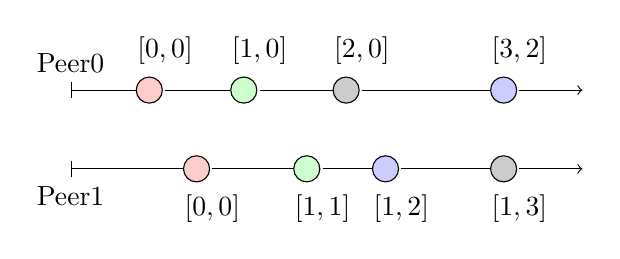
\begin{tikzpicture}

% PEER 0
\draw[|-] (0,1) node[above=1mm]{Peer0} -- (1,1) node{\tikz[baseline]{
	\node[fill=red!20,draw,circle] (f0){};
}};
\draw[-] (1.2,1) node[above=2mm]{$[0,0]$} -- (2.2,1) node{\tikz[baseline]{
	\node[fill=green!20,draw,circle] (f1){};
}};
\draw[-] (2.4,1) node[above=2mm]{$[1,0]$} -- (3.5,1) node{\tikz[baseline]{
	\node[fill=black!20,draw,circle] (f2){};
}};
\draw[-] (3.7,1) node[above=2mm]{$[2,0]$} -- (5.5,1) node{\tikz[baseline]{
	\node[fill=blue!20,draw,circle] (f3){};
}};
\draw[->] (5.7,1) node[above=2mm]{$[3,2]$} -- (6.5,1) node{};

% PEER 1
\draw[|-] (0,0) node[below=1mm]{Peer1} -- (1.6,0) node{\tikz[baseline]{
	\node[fill=red!20,draw,circle] (e0){};
}};
\draw[-] (1.8,0) node[below=2mm]{$[0,0]$} -- (3,0) node{\tikz[baseline]{
	\node[fill=green!20,draw,circle] (e1){};
}};
\draw[-] (3.2,0) node[below=2mm]{$[1,1]$} -- (4,0) node{\tikz[baseline]{
	\node[fill=blue!20,draw,circle] (e2){};
}};
\draw[-] (4.2,0) node[below=2mm]{$[1,2]$} -- (5.5,0) node{\tikz[baseline]{
	\node[fill=black!20,draw,circle] (e3){};
}};
\draw[->] (5.7,0) node[below=2mm]{$[1,3]$} -- (6.5,0) node[below=1mm]{};
\end{tikzpicture}

\begin{tikzpicture}[overlay]
	\path[->] (f1) edge [out=-90, in=135] (e1);
	\path[->] (e2) edge [out=45, in=-135] (f3);
\end{tikzpicture}

  % \caption{An example of a simulation. Red circles are peers' internal events.}
% \end{figure}
